%
% Spark reference architectures
% Copyright (C) 2016 Jan Machacek
%
% This program is free software: you can redistribute it and/or modify
% it under the terms of the GNU General Public License as published by
% the Free Software Foundation, either version 3 of the License, or
% (at your option) any later version.
%
% This program is distributed in the hope that it will be useful,
% but WITHOUT ANY WARRANTY; without even the implied warranty of
% MERCHANTABILITY or FITNESS FOR A PARTICULAR PURPOSE.  See the
% GNU General Public License for more details.
%
% You should have received a copy of the GNU General Public License
% along with this program.  If not, see <http://www.gnu.org/licenses/>.
%

\documentclass[a4paper, 10 pt, conference]{IEEEtran}

\usepackage{graphicx}
\usepackage{interval}
\usepackage{listings}
\usepackage{hyperref}
\usepackage{siunitx}
\usepackage{amsmath}

\sisetup{load-configurations = abbreviations, binary-units = true}
\intervalconfig {
soft open fences ,
separator symbol =; ,
}

\title{Spark Reference Architecture \\ Sensor batch processing}

\author{Jan Mach{\'a}\v{c}ek%$^{1}$% <-this % stops a space
%\thanks{Supported by Cake Solutions Limited}% <-this % stops a space
%\thanks{$^{1}$J. Machacek is the CTO at Cake Solutions, Houldsworth Mill, Houldsworth Street, Reddish, SK5 6DA, UK {\tt\small janm at cakesolutions.net}}%
}


\begin{document}

\maketitle
\thispagestyle{empty}
\pagestyle{empty}

%%%%%%%%%%%%%%%%%%%%%%%%%%%%%%%%%%%%%%%%%%%%%%%%%%%%%%%%%%%%%%%%%%%%%%%%%%%%%%%%
\begin{abstract}

TODO

\end{abstract}


%%%%%%%%%%%%%%%%%%%%%%%%%%%%%%%%%%%%%%%%%%%%%%%%%%%%%%%%%%%%%%%%%%%%%%%%%%%%%%%%
\section{Introduction}

TODO

\section{Reference implementation}

This architecture was used in a connected fitness application. The application processes inputs from one or more sensors (smartwatch, HR sensor, smart clothes) to track fitness regimes and to deliver targeted health and fitness advice to the users. 

The application on the user's smartphone connects data from the available sensors, combines it with a statistical model of the user's behaviour, and---where available---fine-grained location services. These three inputs allow the application to make the first distinction: exercise vs. no-exercise. From the user's perspective, the system is an automated fitness trainer; from a data scientist's perspective, the biometric data the system collects allows for detailed analysis of exercises, exercise regimes, impact of exercise on the users' well-being, automated physiotherapy, and many other applications.

\subsection{Main components}

\begin{figure}[hb]
    \begin{center}
        \caption{Components}
        \label{fig:components}
        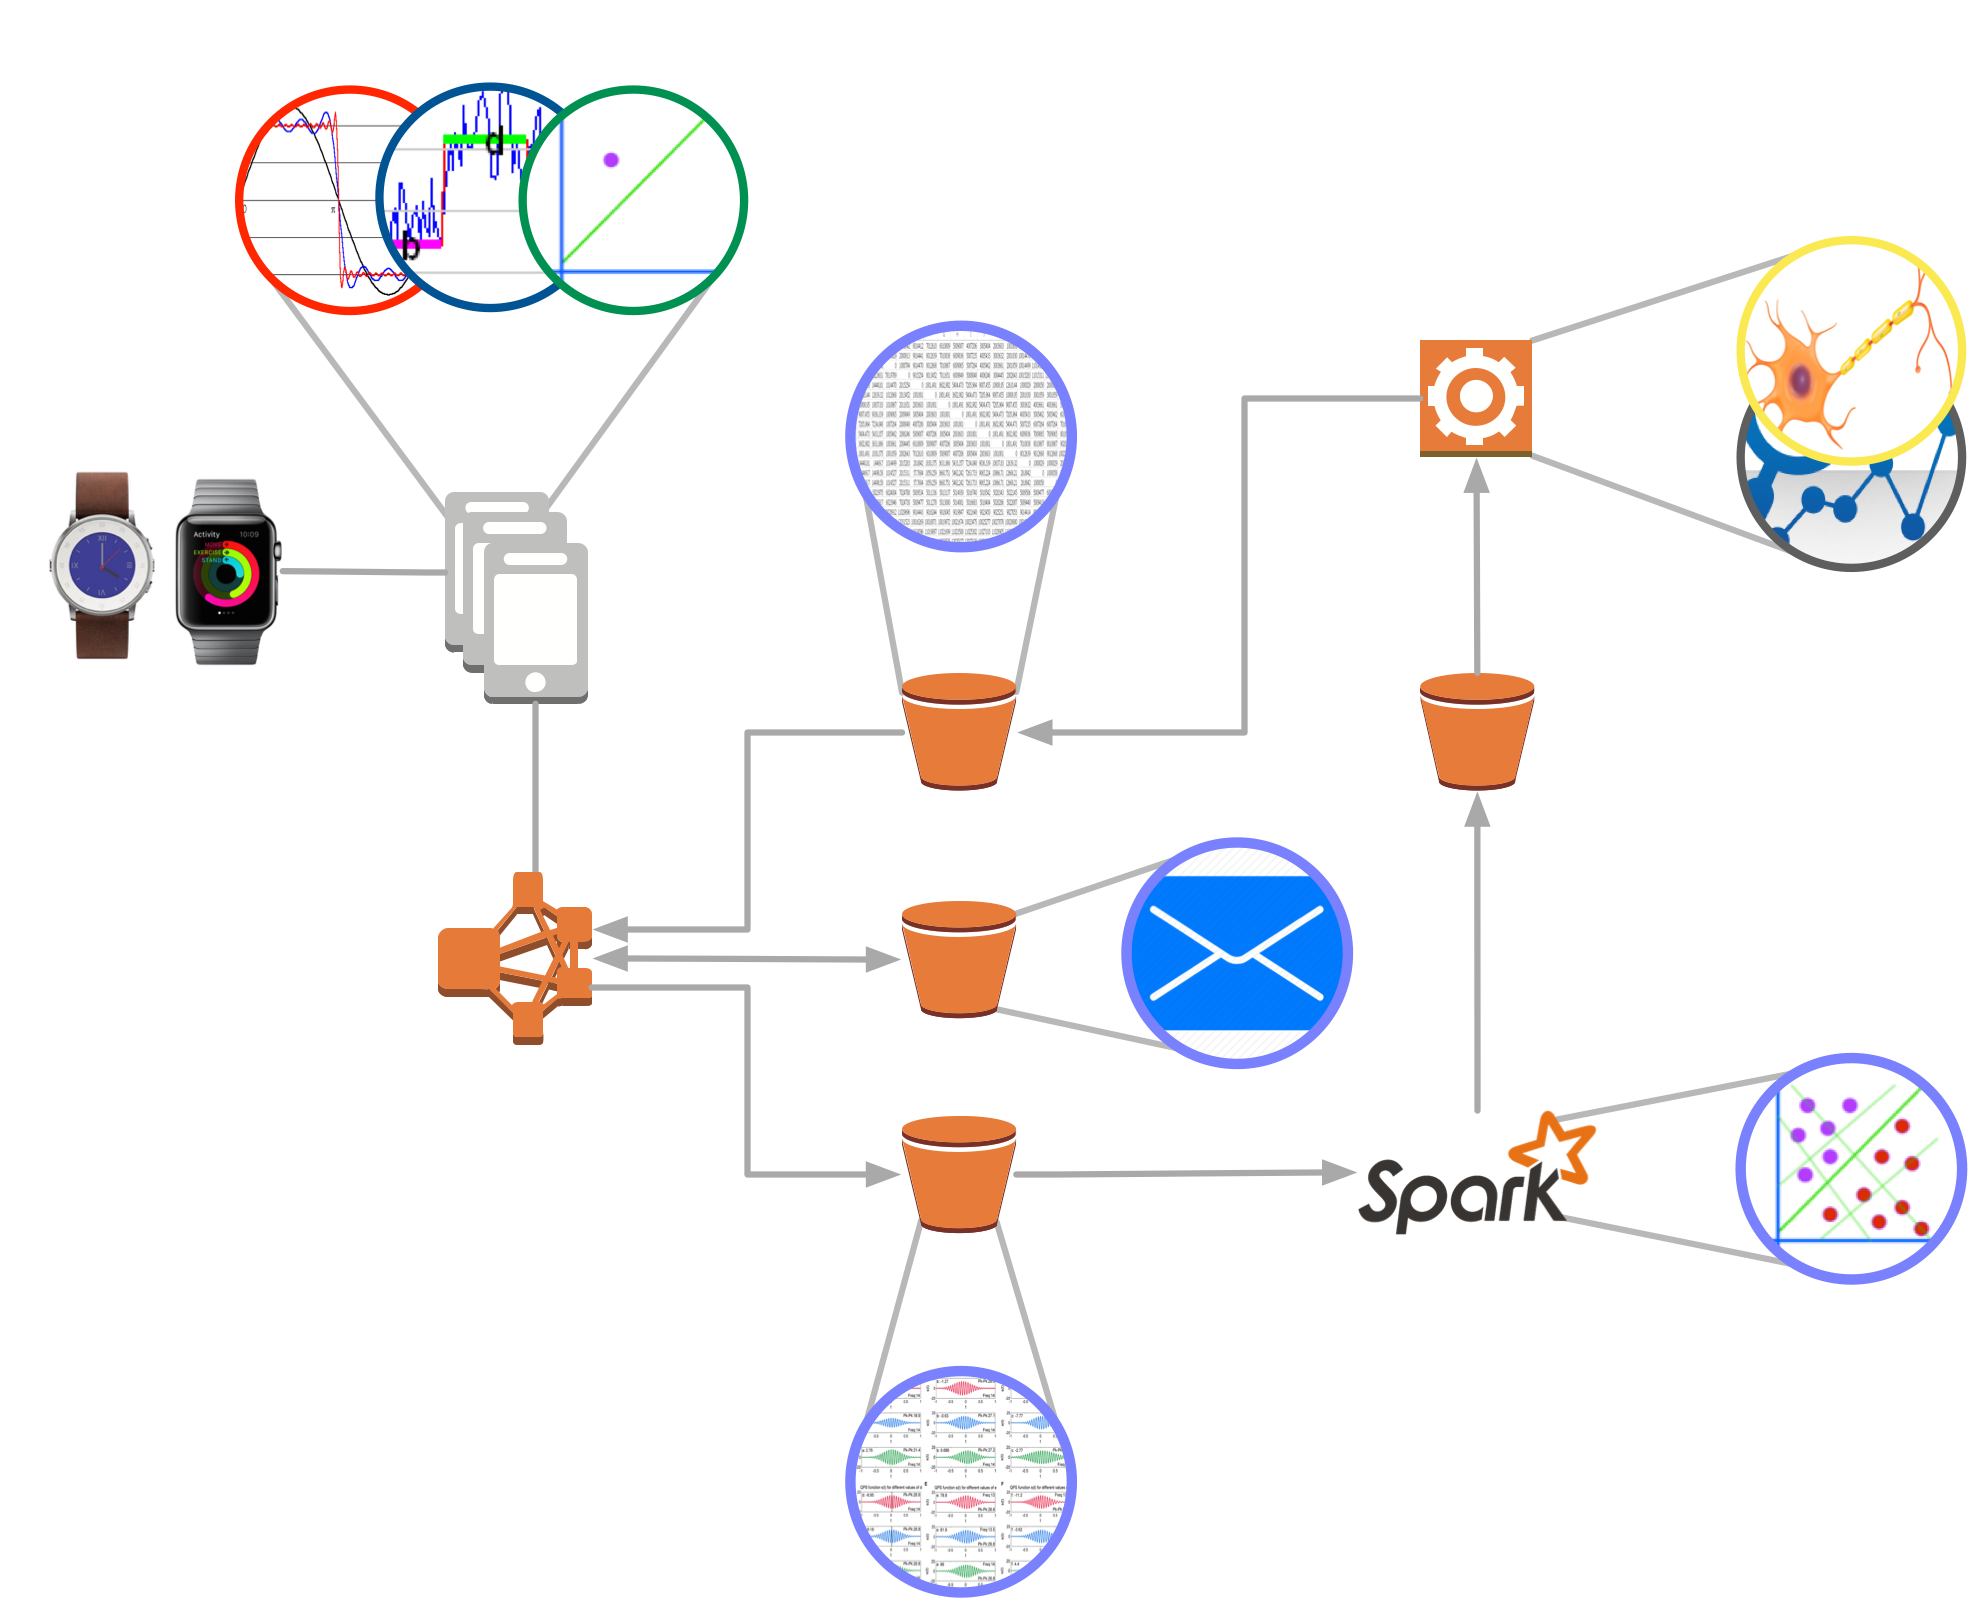
\includegraphics[width=7cm,keepaspectratio]{ri-arch.png}
    \end{center}
\end{figure}

The sensors shown here as consumer-grade wearables perform only the basic hardware interaction: there is no pre-processing of the recorded data. The system accepts accelerometer, gyroscope, heart rate and---where available---data from strain gauges in smart clothes. The mobile application performs the real-time processing of the inputs, displays the next exercise the user should perform (allowing the user to change the suggestion by simply walking to a station for a different exercise, or by beginning a different exercise). The mobile application also prompts the user to confirm correct labels for the recorded data. \emph{This is the key component in the entire system: the frictionless user experience gives the system very accurate labels on very clean data}.

The mobile submits the entire session data (the sensor data, matching labels and latest user behaviour models) in a single request to the Akka \cite{akka} cluster---a CQRS/ES \cite{cqrs-es} microservice implementation. The Akka cluster stores its events and snapshots in a journal, implemented by the Apache Cassandra \cite{apache-cassandra} database. Alongside the events and snapshots, which are opaque to non-Akka systems, the \texttt{exercise} microservice saves the sensor data and the matching labels in a properly formed tabular structure. This structure allows the Apache Spark \cite{apache-spark} cluster to be used for typical big data tasks. An important consideration is privacy and security of the data: the system does not use stable identifiers for the biometric data. This is similar to the unstable advertising identifier used in, for example, the iOS devices \cite{ios-advertising-identifier}. The unstable \emph{biometric identifier} can be refreshed at arbitrary points in time; for very sensitive applications (e.g. clinical physiotherapy), we refresh the biometric identifier after each session; for typical consumer scenarios, we give the users the option to refresh the biometric identifier.

The Apache Spark cluster reads the fitness profiles (associated with the unstable biometric identifier) and computes clusters of users by examining the values in the fitness profile. Even though the profile information holds self-reported data, the data we store include age bracket ($\interval[open]{18}{25}$, $\interval[open]{25}{35}$, $\interval[open]{35}{45}$, ..., $\interval[open]{75}{\inf}$), sex, self-reported fitness level (beginner, intermediate, enthusiast, athlete), self-reported weight and self-reported height.

Once we have the biometric identifiers for each cluster, we read the sensor data, together with the single-session and all-sessions metadata, and find:

\begin{itemize}
\item The Markov chain of exercise sessions that results in greatest improvement (where improvement may be muscle mass gain, fat loss, and \emph{hapiness}.)
\item The Markov chain of exercises in a session that results in greatest improvement (where improvement may be muscle mass gain, fat loss, and \emph{hapiness}.)
\item The most and least popular exercises
\end{itemize}

The output of these \emph{big data} tasks is written back to the Apache Cassandra database; the Akka cluster reads the exercise-related output to provide advice back to the users; the machine learning training and evaluation programs reads the sensor-data related output to compute new models to recognise the exercises.

The models to predict exercise from sensor data are implemented in a cluster of keras \cite{keras} training and evaluation programs. These programs read the sensor data for each cluster, expand the sensor data to each combination of sensors, then train the most successful convolutional neural networks identified through random evolution of previous training executions. (The first execution is human-defined, starting with a three-layer network.) For every sensor data split and every cluster, the training program selects $n$ most successful CNN hyper-parameters from the previous runs, then divides the data into training and test datasets. It then randomly mutates $m$ ($m << n$) CNNs before fitting each CNN to the testing data. The evaluation program then evaluates all new $n$ CNNs, keeping only the most successful ones (defined by the evaluation's F1 score).

The models' hyper-parameters, parameters and evaluation scores are written back to the database. The Akka cluster then selects the best model (hyper-parameters and parameters) and uses the Apple content delivery network to push it to the users with the matching biometric identifiers. (This enables the Akka cluster to concentrate on its primary task: sensor data ingestion, leaving all other data manipulation and transfer tasks to external services while maintaining frictionless user experience.)

\subsection{Mobile application}

The sensors send the data in \SI{1}{\second} batches; the application on the mobile resamples the sampling rate to \SI{50}\hertz. (Accelerometer and gyroscope typically sample at this rate, heart rate and the strain gauges in smart clothes can be up-sampled to \SI{50}{\hertz} easily.) The mobile application ingests the data from the sensors and, together with a statistical model of the user's short-term behaviour, attempts to identify the movement. The models in the mobile application can make successful predictions of sequence of exercises in a session and the properties of each exercise (i.e. weight, number of repetitions, duration, intensity). The model used to predict sequence of exercise sessions and exercises within a session is a Markov chain \cite{markov-chain-exercise}. This approach allows the application to deal with the reality of exercise in a public gym, where the station for the next suggested exercise might not be available. The Markov chain, together with a bio-mechanical model of the main muscle groups, gives the users the flexibility to achieve their workout targets even in crowded gyms. The sequence of exercise predictions for one particular exercise sessions are illustrated on \autoref{fig:model-sequence}.

\begin{figure}[h]
    \begin{center}
        \caption{Exercise sequence model with no context}
        \label{fig:model-sequence}
        
\includegraphics[width=7cm,keepaspectratio]{ri-model-sequence.png}
    \end{center}
\end{figure}

The numbers in \autoref{fig:model-sequence} represent the count of transitions taken; hence it is possible to calculate the probability of transition from any given state. The state names represent the exercise labels, in real application, they are the real exercise names. The mobile application can either receive the chain when the user selects one of the pre-defined exercise programmes, or it can construct the chain from empty if the user choses to start his or her custom workout. This gives the application an intuitive feel; its suggestions are what the users usually do. Finally, the information in the chain allows the system to identify the most popular sequences of exercises, to identify exercises that the users do not like; more interestingly, the system can use the information in the chain to identify sequence of exercises that leads to the best improvement. (At this point, we do not define what the improvement is: in some applications, it may be weight loss; in other applications, it may be greatest mobility range improvement; and many others.)

To make the next-exercise prediction more accurate, the mobile application uses fined-grained location services. The location services are implemented using bluetooth beacons. The beacons operate in the iBeacon mode \cite{ibeacon}; each beacon in this mode transmits its identifier, a major, and minor values. The mobile application sets up continuous scanning of a major value which identifies exercise equipment, receiving notifications of beacons and their minor values as they come into range. The mobile application then filters the exercise states keeping only those that are associated with a particular area. (Viz \autoref{fig:model-sequence+location}.)

\begin{figure}[h]
    \begin{center}
        \caption{Exercise sequence model with location context}
        \label{fig:model-sequence+location}
        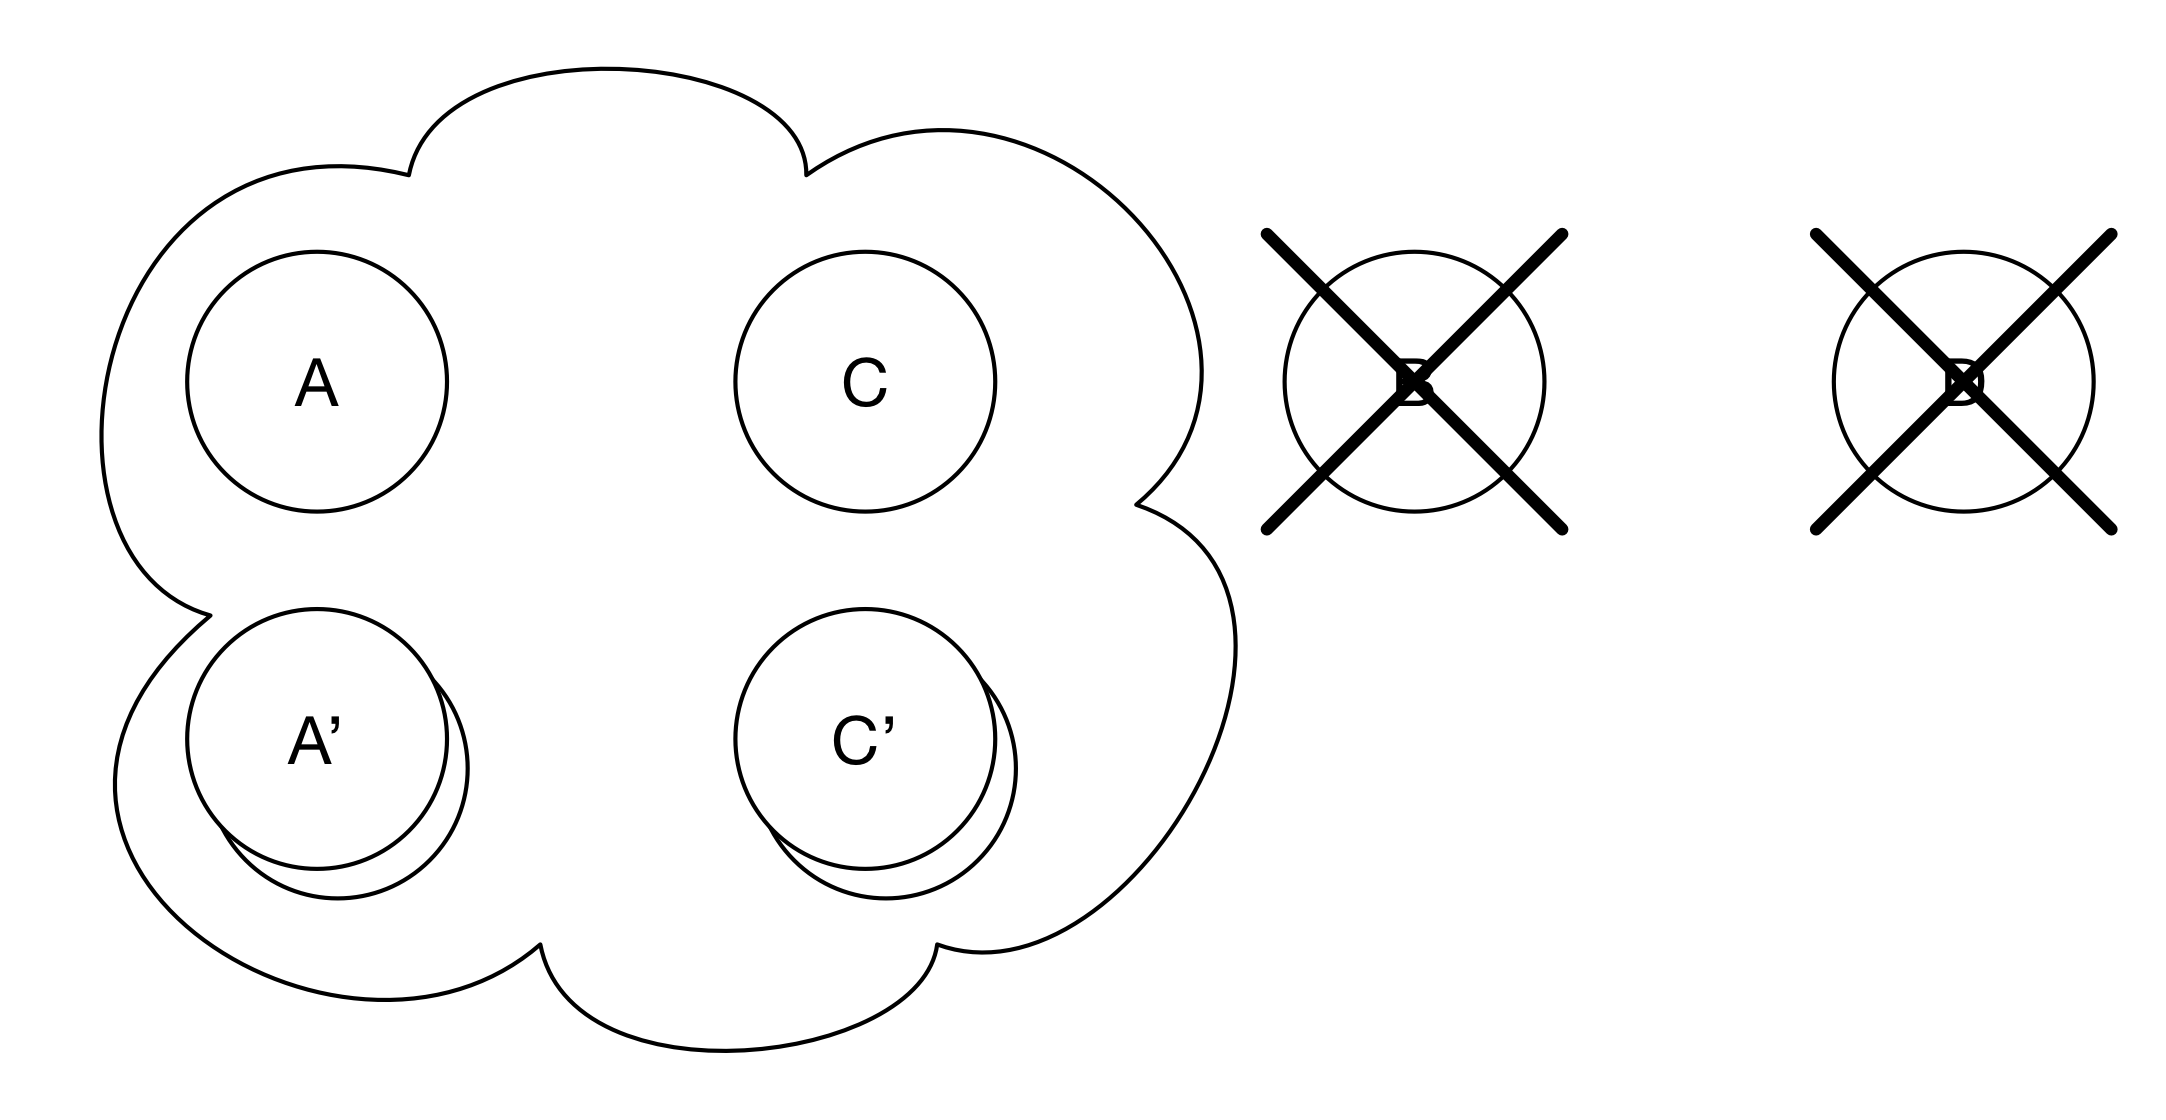
\includegraphics[width=7cm,keepaspectratio]{ri-model-sequence+location.png}
    \end{center}
\end{figure}

With the fine-grained location data available, the application is \emph{expecting} to see a movement that precedes exercises A or C. We call this movement the \emph{setup movement}. The setup movement classifier is a multi-layer perceptron, which takes \SI{1}\second of sensor input and produces probabilities classes that represent the setup movement for groups of exercises. The hyper-parameters of the MLP is driven by the sensor data as its inputs; for example, accelerometer-only MLP has 150 inputs (50 samples of the acceleration vector) and as many outputs as the number of recognised setup movements. It is important to measure and optimise the power requirements for the computation; on iOS, we took advantage of the vDSP and veclib frameworks, which offer optimised vector operations. The MLP classes are not the exercises themselves, but the setup movements; one setup movement can map to multiple exercises. To provide accurate prediction of the exercise about to be started, the mobile application takes into account the expected exercise (given the user's typical behaviour), and the fine-grained location data. The performance of the exercise prediction for accelerometer on the user's wrist is shown in \autoref{tbl:setup-movement-performance-accelerometer}; the performance of the exercise prediction rises significantly in fully-wired human (viz \autoref{tbl:setup-movement-performance-all}).

\begin{table}[h]
\caption{Exercise prediction performance (accelerometer)}
\label{tbl:setup-movement-performance-accelerometer}
\begin{center}
\begin{tabular}{|l||m{1cm}|m{1cm}|m{1cm}|m{1cm}|}
\hline                      & Accuracy & Precision & Recall & F1 \\
\hline No context           & !!       & !!        & !!     & !! \\
\hline Behaviour            & !!       & !!        & !!     & !! \\ 
\hline Behaviour + Location & !!       & !!        & !!     & !! \\
\hline
\end{tabular}
\end{center}
\end{table}

\begin{table}[h]
\caption{Exercise prediction performance (all sensors)}
\label{tbl:setup-movement-performance-all}
\begin{center}
\begin{tabular}{|l||m{1cm}|m{1cm}|m{1cm}|m{1cm}|}
\hline                      & Accuracy & Precision & Recall & F1 \\
\hline No context           & !!       & !!        & !!     & !! \\
\hline Behaviour            & !!       & !!        & !!     & !! \\ 
\hline Behaviour + Location & !!       & !!        & !!     & !! \\
\hline
\end{tabular}
\end{center}
\end{table}

Finally, the mobile application asks the user to confirm the label for the collected sensor data. Given the good performance of the exercise recognition (particularly when using fine-grained location services), this is typically just a \emph{confirm} step rather than complex data entry exercise. The mobile application builds a local store of the time regions of labelled sensor data. This store, together with the Markov chain representing the exercise sequence and the final feedback (happy, indifferent, unhappy) is submitted to the server. The server decompresses \& decodes the submitted data and stores it in tabular form in Apache Cassandra, referencing the user's biometric ID. 

\section{Server components}

The Akka cluster is a CQRS/ES system, which exposes REST APIs for the mobile application. The REST requests it receives are treated as commands; once a command is validated, the code in the cluster turns it into an \emph{event} and persists it in the journal. Later on, another component may represent the system's state as the sum of all the events in the journal. This \emph{command / query responsibility separation} approach makes it possible to efficiently distribute the processing required by the system's components. (For example, if the users often request a view of the state of the system, then the \emph{query} components receive more resources.) The Akka toolkit uses Actor-based concurrency: within an actor, all computation is synchronous; the toolkit handles asynchronous communication between actors. This allows us to maintain clear boundary on any mutable state: if is kept within an actor, it is safe. 

\section{Apache Spark batch analytics}

Vivamus urna velit, volutpat ut tincidunt sit amet, pulvinar vitae est. Nam tortor sapien, sagittis non luctus sit amet, porttitor a purus. Donec mattis blandit bibendum. Morbi ipsum lacus, gravida ut nibh semper, porta tincidunt ex. Sed tellus lectus, posuere in facilisis quis, suscipit eu tortor. Maecenas sagittis diam non orci scelerisque, vehicula rutrum ipsum elementum. Lorem ipsum dolor sit amet, consectetur adipiscing elit. Proin bibendum justo gravida sem accumsan consequat. Nunc tristique aliquam magna, id convallis tellus gravida et. Sed orci est, tempus eu ligula sed, posuere feugiat nunc. Sed est mauris, dignissim dignissim pretium in, elementum a neque. Phasellus mollis sollicitudin justo, ut commodo turpis volutpat in. Fusce egestas nunc dui, vel mollis tellus interdum vel. Donec porttitor lorem non mauris porttitor, euismod vestibulum nisi tincidunt. Nunc fringilla risus nulla, id vulputate sem blandit ut. Proin est mauris, viverra in interdum quis, fringilla at augue.

Vivamus urna velit, volutpat ut tincidunt sit amet, pulvinar vitae est. Nam tortor sapien, sagittis non luctus sit amet, porttitor a purus. Donec mattis blandit bibendum. Morbi ipsum lacus, gravida ut nibh semper, porta tincidunt ex. Sed tellus lectus, posuere in facilisis quis, suscipit eu tortor. Maecenas sagittis diam non orci scelerisque, vehicula rutrum ipsum elementum. Lorem ipsum dolor sit amet, consectetur adipiscing elit. Proin bibendum justo gravida sem accumsan consequat. Nunc tristique aliquam magna, id convallis tellus gravida et. Sed orci est, tempus eu ligula sed, posuere feugiat nunc. Sed est mauris, dignissim dignissim pretium in, elementum a neque. Phasellus mollis sollicitudin justo, ut commodo turpis volutpat in. Fusce egestas nunc dui, vel mollis tellus interdum vel. Donec porttitor lorem non mauris porttitor, euismod vestibulum nisi tincidunt. Nunc fringilla risus nulla, id vulputate sem blandit ut. Proin est mauris, viverra in interdum quis, fringilla at augue.

Vivamus urna velit, volutpat ut tincidunt sit amet, pulvinar vitae est. Nam tortor sapien, sagittis non luctus sit amet, porttitor a purus. Donec mattis blandit bibendum. Morbi ipsum lacus, gravida ut nibh semper, porta tincidunt ex. Sed tellus lectus, posuere in facilisis quis, suscipit eu tortor. Maecenas sagittis diam non orci scelerisque, vehicula rutrum ipsum elementum. Lorem ipsum dolor sit amet, consectetur adipiscing elit. Proin bibendum justo gravida sem accumsan consequat. Nunc tristique aliquam magna, id convallis tellus gravida et. Sed orci est, tempus eu ligula sed, posuere feugiat nunc. Sed est mauris, dignissim dignissim pretium in, elementum a neque. Phasellus mollis sollicitudin justo, ut commodo turpis volutpat in. Fusce egestas nunc dui, vel mollis tellus interdum vel. Donec porttitor lorem non mauris porttitor, euismod vestibulum nisi tincidunt. Nunc fringilla risus nulla, id vulputate sem blandit ut. Proin est mauris, viverra in interdum quis, fringilla at augue.


\section{Machine learning}

The ML training and evaluation programs use Python and run in Docker containers. To support fast development cycle, we build two flavours of Docker images: a \emph{light} image that can run on nearly any underlying hardware, and a CUDA \cite{cuda} image that runs on the EC2 \texttt{g2.2xlarge} instance.

Glossing over some important details, its execution is the following loop:

\begin{itemize}
\item Generate new model hyperparameters by appending randomly mutated hyperparameters to the current set of hyperparameters,
\item For each model hyperparameters, construct a model and fit the training dataset,
\item Measure the fitted model's performance using the test dataset,
\item Save the measured performance and hyperparameters
\end{itemize}

The hyperparameter mutating code is fairly basic at the moment; it can only
\begin{itemize}
\item Mutate dense layer's activation functions
\item Mutate dropout layer's rate
\item Mutate convolution layer's kernel
\item Remove or add layer
\item Mutate learning rate, momentum and and decay of the SGD optimiser
\end{itemize}

Notice also that our evolution code is purely random; there is no optimiser. This code does produce well-performing models, though \emph{its energy or cost efficiency is extremely poor}. \autoref{fig:ri-model-evolution} illustrates this process for 2 models hyperparameters.

\begin{figure}[h]
    \begin{center}
        \caption{Model evolution}
        \label{fig:ri-model-evolution}
        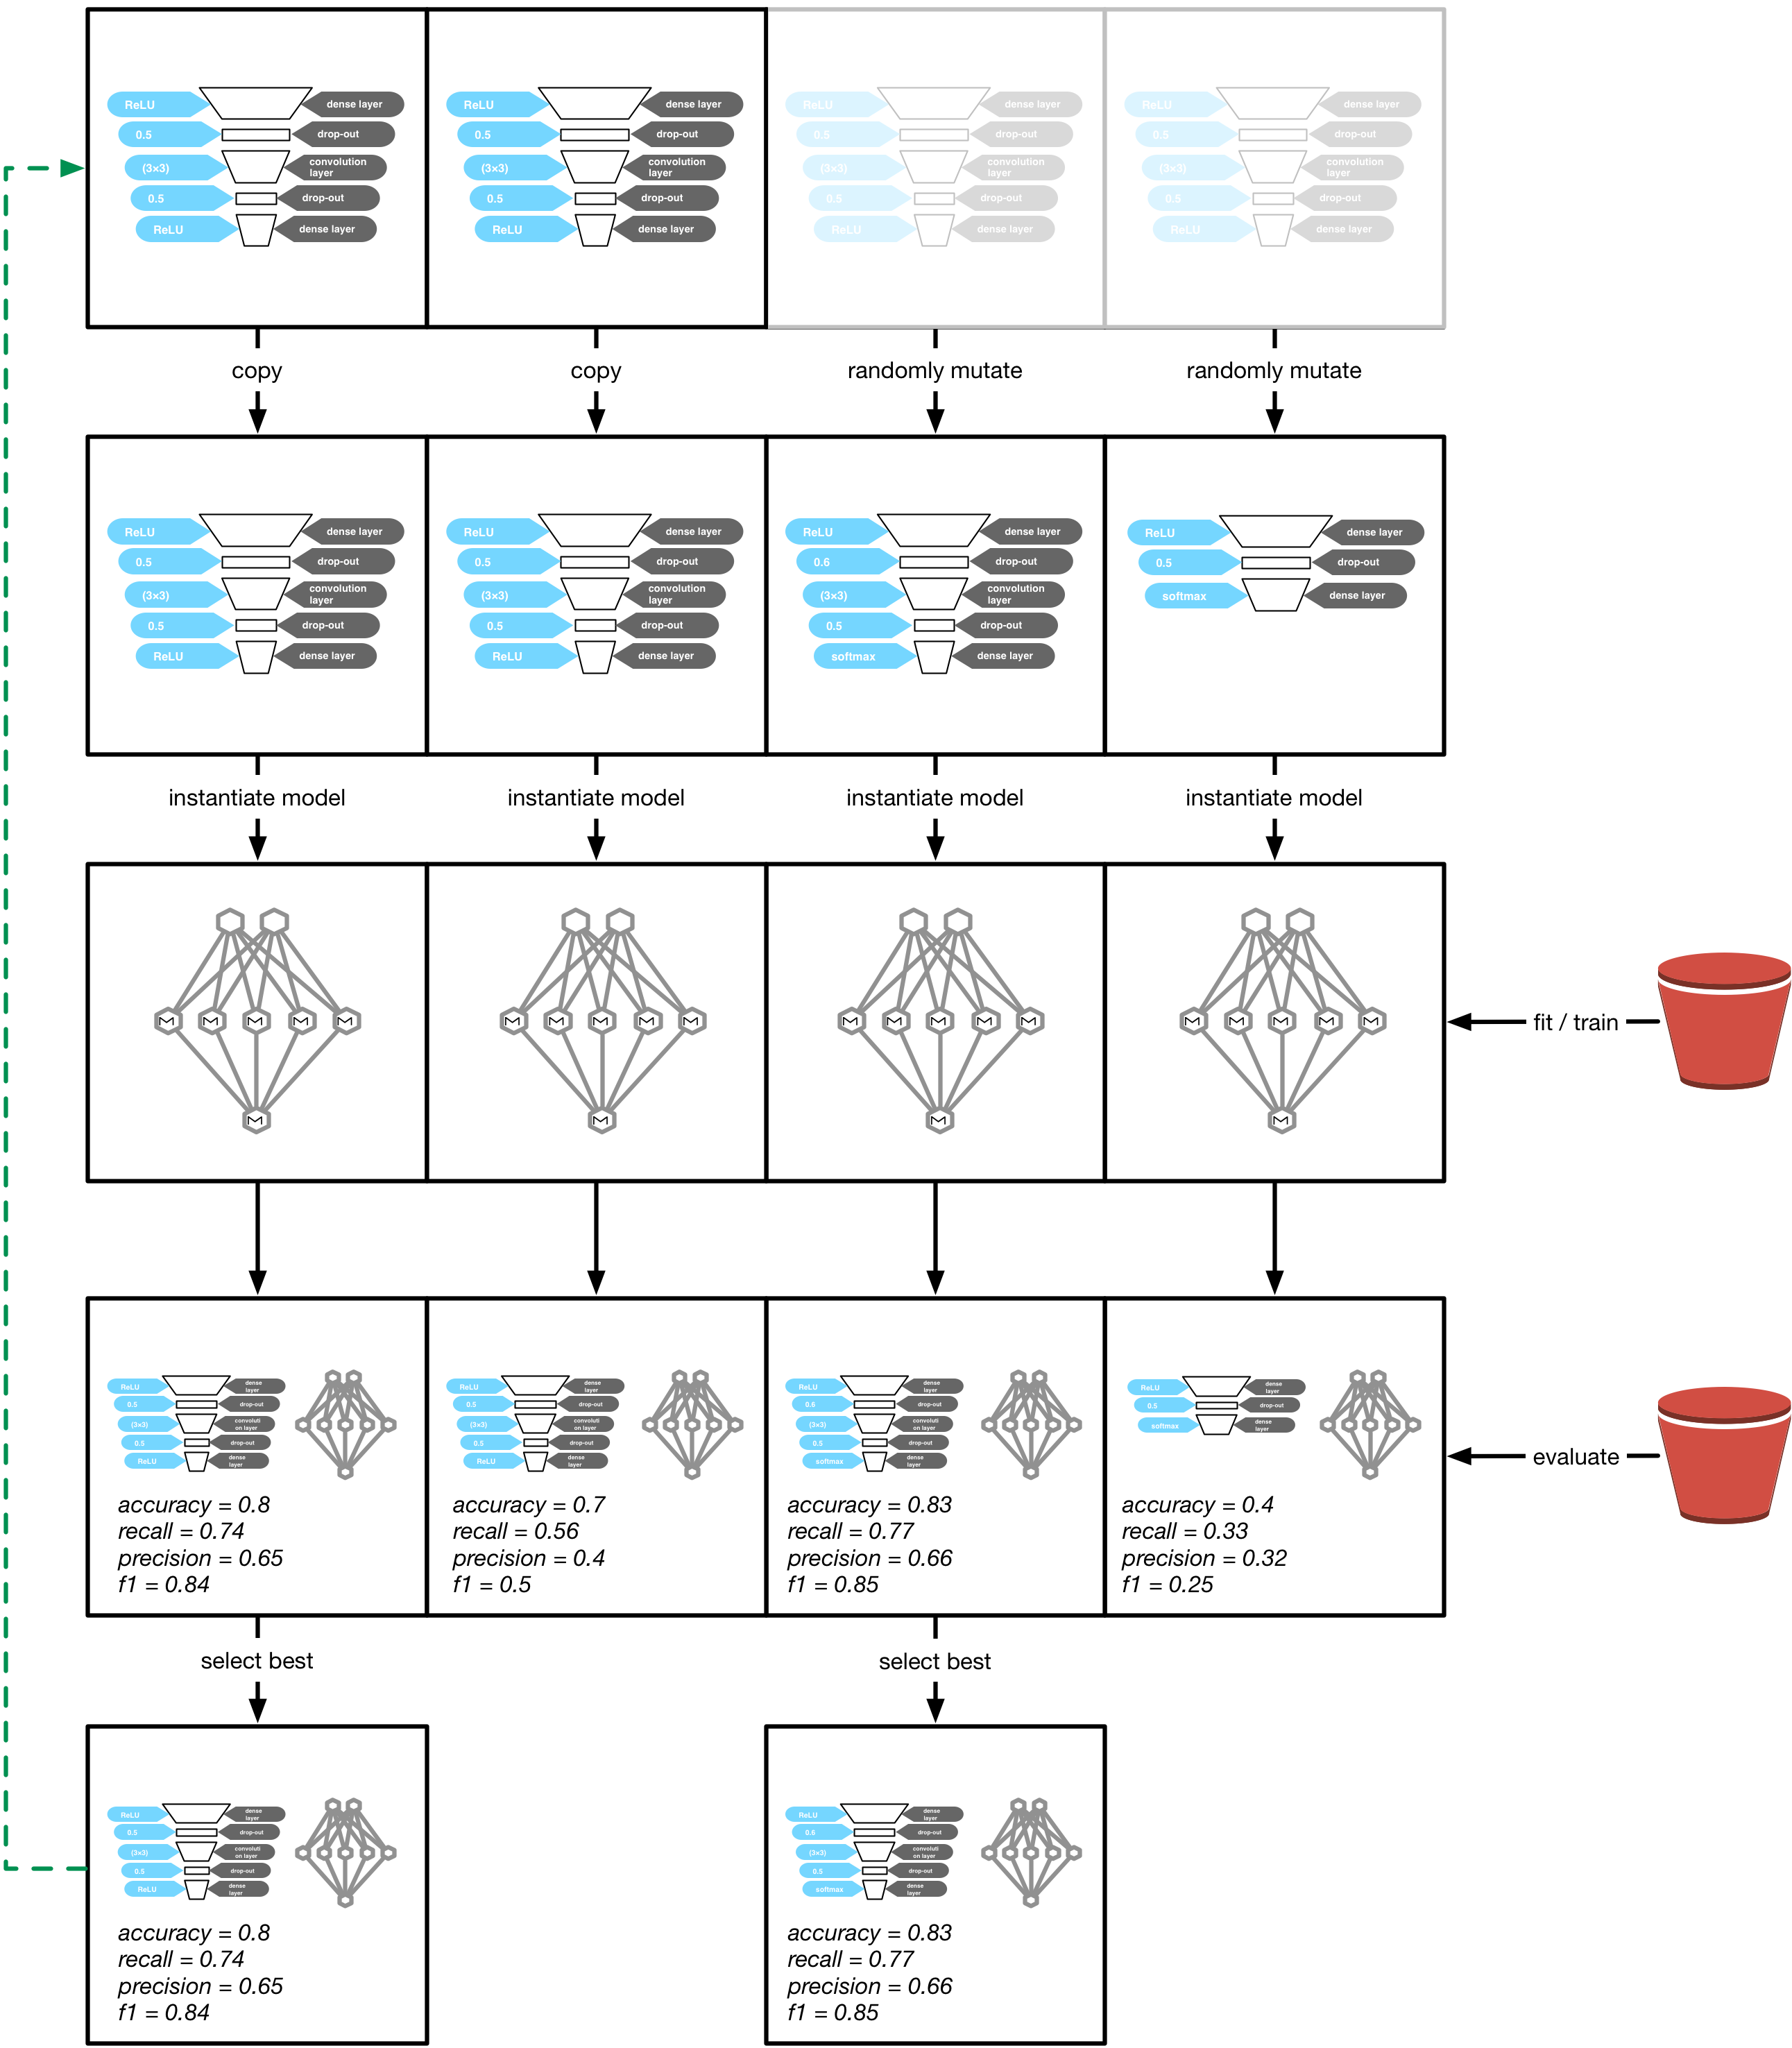
\includegraphics[width=7cm,keepaspectratio]{ri-model-evolution.png}
    \end{center}
\end{figure}

The final consideration is the sensor data explosion: this is something that we actually need in our system to be able to make as much of the collected data as possible. While most users wear only a single smartwatch (which gives us accelerometer data from one wrist), there are some users who wear many more sensors. What we call a \emph{fully-wired human} wears accelerometer and gyroscope on the wirst, together heart rate monitor and sports clothes that contain strain gauges along major muscle groups. This gives us (at the moment) 2 data points from the wrist, 1 from the heart rate sensor (we drop down to simple heart rate, we do not measure the full ECG traces), and \emph{20 data points from the muscle groups}. Just under \SI{50}{\percent} of our users fall somewhere between the smartwatch-only and fully-wired categories. To ensure that we make the most of every user, the training program needs to expand the recorded data into all known sensor combinations. So, for a dataset with $n$ sensors, we expand it into $\binom nn + \binom n{n-1} + \binom n{n-2} + ... + \binom n1$ datasets.



Vivamus urna velit, volutpat ut tincidunt sit amet, pulvinar vitae est. Nam tortor sapien, sagittis non luctus sit amet, porttitor a purus. Donec mattis blandit bibendum. Morbi ipsum lacus, gravida ut nibh semper, porta tincidunt ex. Sed tellus lectus, posuere in facilisis quis, suscipit eu tortor. Maecenas sagittis diam non orci scelerisque, vehicula rutrum ipsum elementum. Lorem ipsum dolor sit amet, consectetur adipiscing elit. Proin bibendum justo gravida sem accumsan consequat. Nunc tristique aliquam magna, id convallis tellus gravida et. Sed orci est, tempus eu ligula sed, posuere feugiat nunc. Sed est mauris, dignissim dignissim pretium in, elementum a neque. Phasellus mollis sollicitudin justo, ut commodo turpis volutpat in. Fusce egestas nunc dui, vel mollis tellus interdum vel. Donec porttitor lorem non mauris porttitor, euismod vestibulum nisi tincidunt. Nunc fringilla risus nulla, id vulputate sem blandit ut. Proin est mauris, viverra in interdum quis, fringilla at augue.

Vivamus urna velit, volutpat ut tincidunt sit amet, pulvinar vitae est. Nam tortor sapien, sagittis non luctus sit amet, porttitor a purus. Donec mattis blandit bibendum. Morbi ipsum lacus, gravida ut nibh semper, porta tincidunt ex. Sed tellus lectus, posuere in facilisis quis, suscipit eu tortor. Maecenas sagittis diam non orci scelerisque, vehicula rutrum ipsum elementum. Lorem ipsum dolor sit amet, consectetur adipiscing elit. Proin bibendum justo gravida sem accumsan consequat. Nunc tristique aliquam magna, id convallis tellus gravida et. Sed orci est, tempus eu ligula sed, posuere feugiat nunc. Sed est mauris, dignissim dignissim pretium in, elementum a neque. Phasellus mollis sollicitudin justo, ut commodo turpis volutpat in. Fusce egestas nunc dui, vel mollis tellus interdum vel. Donec porttitor lorem non mauris porttitor, euismod vestibulum nisi tincidunt. Nunc fringilla risus nulla, id vulputate sem blandit ut. Proin est mauris, viverra in interdum quis, fringilla at augue.

Vivamus urna velit, volutpat ut tincidunt sit amet, pulvinar vitae est. Nam tortor sapien, sagittis non luctus sit amet, porttitor a purus. Donec mattis blandit bibendum. Morbi ipsum lacus, gravida ut nibh semper, porta tincidunt ex. Sed tellus lectus, posuere in facilisis quis, suscipit eu tortor. Maecenas sagittis diam non orci scelerisque, vehicula rutrum ipsum elementum. Lorem ipsum dolor sit amet, consectetur adipiscing elit. Proin bibendum justo gravida sem accumsan consequat. Nunc tristique aliquam magna, id convallis tellus gravida et. Sed orci est, tempus eu ligula sed, posuere feugiat nunc. Sed est mauris, dignissim dignissim pretium in, elementum a neque. Phasellus mollis sollicitudin justo, ut commodo turpis volutpat in. Fusce egestas nunc dui, vel mollis tellus interdum vel. Donec porttitor lorem non mauris porttitor, euismod vestibulum nisi tincidunt. Nunc fringilla risus nulla, id vulputate sem blandit ut. Proin est mauris, viverra in interdum quis, fringilla at augue.

\section{Server infrastructure}

To run the system's server components, a modern cluster management \& distributed init system abstracting over a fault-tolerant, self-healing infrastructure is needed. In our case, a highly available Mesos \cite{mesos} cluster provides abstraction at the datacentre level and acts as a datacentre-wide resource manager. To achieve faster deployments, the microservices that comprise the system are packaged as Docker \cite{docker} images. The build system (Jenkins \cite{jenkins}) starts by building the Docker images. These images are deployed and managed using a scheduler (Marathon \cite{marathon}) which acts as the distributed init system and the process manager. Marathon is used for long-running jobs such as the microservices, and the database cluster; Chronos \cite{chronos} is used to manage the short-lived jobs (e.g. the batching Apache Spark jobs). Having Marathon and Chronos job configurations in git allows for any changes to infrastructure to be versioned, traceable and auditable. Job configuration changes are synchronised to a distributed key-value store (Consul \cite{consul}). When a job configuration changes, the Consul handler uses the scheduler API (Marathon REST API) to trigger the infrastructure update through the cluster OS (Mesos). Finally, the cluster OS metrics and the list of running services from the service registry provide the information for the dynamic scaling code.
This infrastructure allowed us to implement and maintain a robust and reliable production system. \autoref{fig:infrastructure} illustrates the outline of our cloud-based infrastructure and highlights the workflow of putting code to production.

\begin{figure}[h]
    \begin{center}
        \caption{Infrastructure diagram}
        \label{fig:infrastructure}
        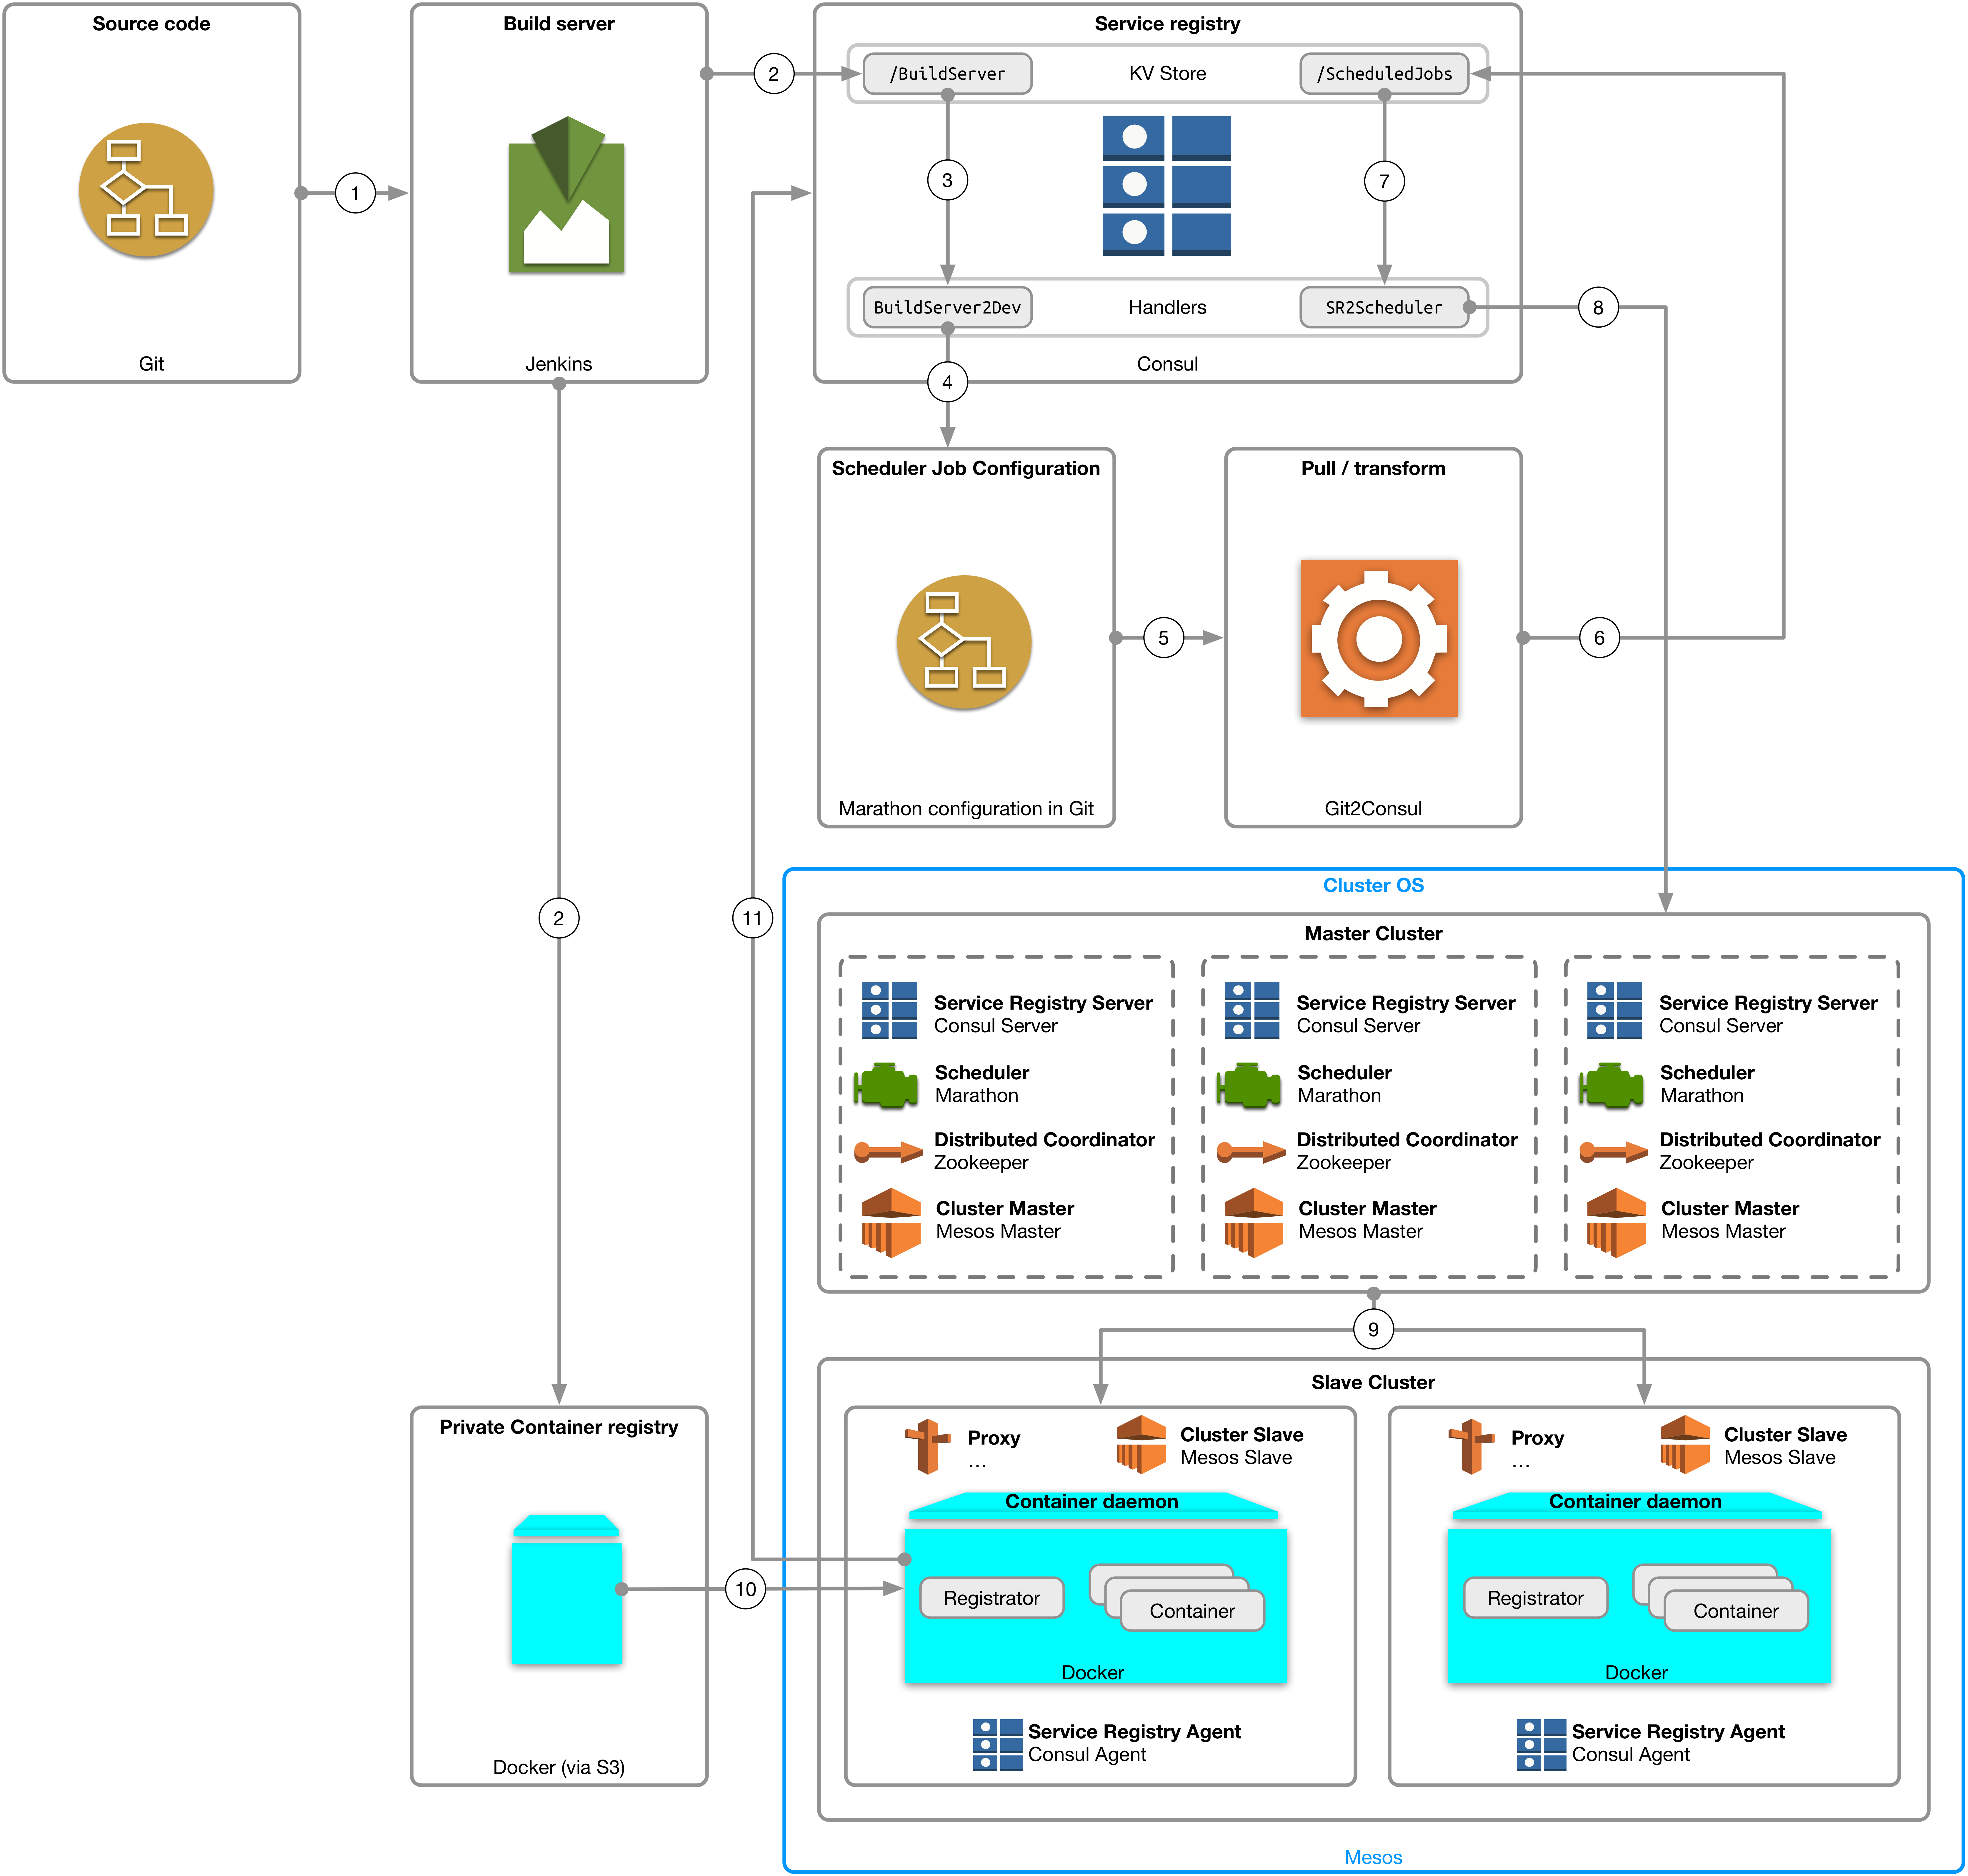
\includegraphics[width=7cm,keepaspectratio]{ri-infrastructure.png}
    \end{center}
\end{figure}

There are many more topics that we could not describe here: rolling upgrades without message loss, zero downtime deployment, message versioning, API versioning, message integrity verification, detailed privacy and security concerns, wire formats, cluster consistencies, reliable multi-region and global implementations, test and training data management, model evolution, centralized logging, back pressure reporting and handling, and many more. 

\section{Further research}

We are also very excited to use this work as a basis for a Horizon 2020 \cite{horizon2020} project proposal; the aim of the Horizon 2020 project is to help as many people as possible to help become more active, while at the same time preventing injury; to assist with weight management (which is particularly difficult due to self-reporting of the food consumption, but is possible to approach thanks to modern payment instruments like Mondo \cite{mondo}). Finally, it might be possible to assist with physiotherapy, but that will require identifying not only the exercise class, but to also be able to measure \emph{quality} of the exercise class.

Further research will focus on the system's human interaction. Interacting with a screen while exercising greatly reduces the effort the users put in \cite{!!!}; however, listening to music often has the opposite effect \cite{!!!}. Therefore, our future research will explore conversational interfaces delivered through voice synthethiser. 

\section{Summary}

The focus of our work is on guiding the user during his or her exercise or physiotherapy session; to do that, it is necessary to indicate to the user \emph{what to do next} and to recognise that the exercise is actually being performed, and to give feedback about the exercise being performed, as early as possible. In our testing, we found that delays of more than \SI{1}{\second} confuse the users. It was not possible to use the work in \cite{morris:2014ir}; instead, we needed to build our own probabilistic model of next exercise and then eager sensor data recognition layer. It is equally important to accurately collect labelled data, this is achieved through frictionless user interface. The labelled sensor data, the exercise sequences, and the feedback data is written---together with the matching unstable biometric ID and associated profile---to a Apache Cassandra database in normal tabular form. The Apache Spark jobs then identify clusters of biometric IDs based on the information in the profiles, together with (per cluster) the best sequence of exercises and the best sequence of exercise sessions, the top $n$ user-contributed exercises.

\addtolength{\textheight}{-12cm}  % This command serves to balance the column lengths
                                  % on the last page of the document manually. It shortens
                                  % the textheight of the last page by a suitable amount.
                                  % This command does not take effect until the next page
                                  % so it should come on the page before the last. Make
                                  % sure that you do not shorten the textheight too much.

\begin{thebibliography}{99}

\bibitem{markov-chain-exercise} F. Oo, Q. Uux. Bar. 2016.
\bibitem{akka} Akka.
\bibitem{cqrs-es} CQRS/ES.
\bibitem{apache-cassandra} Apache Cassandra.
\bibitem{apache-spark} Apache Spark.
\bibitem{ibeacon} iBeacon.
\bibitem{ios-advertising-identifier} iOS advertising identifier.
\bibitem{keras} keras.
\bibitem{mesos} Mesos.
\bibitem{jenkins} Jenkins.
\bibitem{marathon} Marathon.
\bibitem{docker} Docker.
\bibitem{chronos} Chronos.
\bibitem{consul} Consul.
\bibitem{horizon2020} European Commission. Horizon 2020. https://ec.europa.eu/programmes/horizon2020/. 28 May 2016.

\bibitem{mondo} Mondo.
\bibitem{cuda} CUDA.
\bibitem{morris:2014ir} Morris, D., Saponas, T. S., Guillory, A., \& Kelner, I. (2014). RecoFit (pp. 3225--3234). Presented at the the 32nd annual ACM conference, New York, New York, USA: ACM Press. http://doi.org/10.1145/2556288.2557116

\end{thebibliography}


\end{document}
